\documentclass{article}
\usepackage{graphicx} 
\usepackage{multirow}
\usepackage{multicol}
\usepackage{enumitem}
\usepackage{amssymb}
\usepackage{amsmath}
\usepackage{xcolor}
\usepackage{cancel}
\usepackage{tcolorbox}
\usepackage{geometry}
\usepackage{tikz}
\usepackage{tikz-3dplot}
\usepackage{pgfplots, tkz-euclide,calc}
    \usetikzlibrary{patterns,snakes,shapes.arrows,3d}
    \usepgfplotslibrary{fillbetween}
	\geometry{
		total = {160mm, 237mm},
		left = 25mm,
		right = 35mm,
		top = 30mm,
		bottom = 30mm,
	}

\newcommand{\jawab}{\textbf{Solution}:}
\newcommand{\del}{\partial}
\begin{document}
    \pagenumbering{gobble}
    \begin{tabular}{|lcl|}
     \hline
     Nama&:&Teosofi Hidayah Agung\\
     NRP&:&5002221132\\
     \hline
    \end{tabular}
    \begin{enumerate}
        \item[19.] Let $X$ and $Y$ be continuous random variables with joint pdf of the form
        \[f(x,y)=k(x+y)\quad 0\leq x\leq y\leq 1\]
        and zero otherwise.
        \begin{enumerate}
            \item Find the value of $k$.\\
            \jawab\\
            The region of pdf can be seen in the following figure.
            \begin{center}
                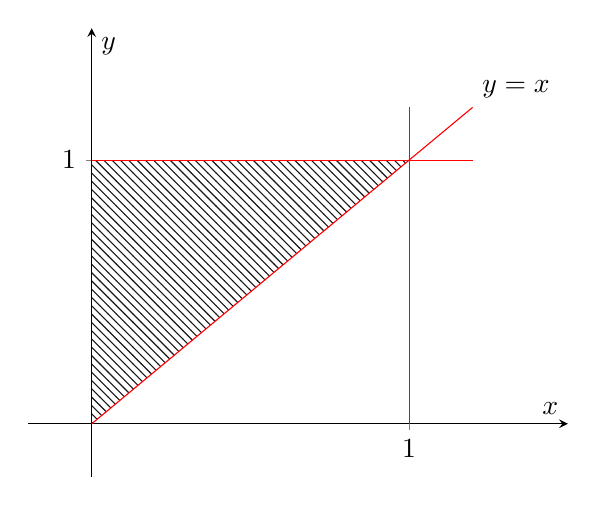
\begin{tikzpicture}
                    \begin{axis}[axis lines = center, xlabel = $x$, ylabel = $y$, xmin = -0.2, xmax = 1.5, ymin = -0.2, ymax = 1.5,xtick={1},
                        ytick={1}]
                        \addplot [
                            domain=0:1.2, 
                            samples=100, 
                            color=red,
                            name path=A,
                        ]
                        {x} node[pos=1.0](endofplotsquare){} ;
                        \node [above right] at (endofplotsquare) {$y=x$};
                        \addplot [
                            domain=0:1.2, 
                            samples=10, 
                            color=red,
                            name path=B,
                        ]
                        {1} node[pos=0.75](endofplotsquare){} ;
                        \node [above left] at (endofplotsquare) {};
                        \addplot[samples=10, smooth,domain=1:2,red] coordinates {(1,0)(1,1.2)};
                        \addplot[fill=gray,opacity=0.9,pattern=north west lines,line width=1pt] fill between[of=A and B,split,soft clip={domain=0:1}];
                    \end{axis}
                \end{tikzpicture}
            \end{center}
            So the value of $k$ can be found by integrating the pdf over that region.
            \begin{flalign*}
                \int_{-\infty}^\infty\int_{-\infty}^\infty f(x,y)\,dx\,dy&=1\\
                \int_0^1\int_0^y k(x+y)\,dx\,dy&=1\\
                k\int_0^1\left[\frac{x^2}{2}+xy\right]^y_0\,dy&=1\\
                k\int_0^1\left(\frac{y^2}{2}+y^2\right)\,dy&=1\\
                k\left[\frac{y^3}{6}+\frac{y^3}{3}\right]_0^1&=1\\
                k\left(\frac{1}{6}+\frac{1}{3}\right)&=1\\
                k\left(\frac{1}{6}+\frac{2}{6}\right)&=1\\
                k\left(\frac{1}{2}\right)&=1\\
                k&=2
            \end{flalign*}
            \item Find the marginals, $f_1(x)$ and $f_2(y)$.\\
            \jawab
            \begin{multicols}{2}
                \noindent
                \begin{flalign*}
                    f_1(x)&=\int_{-\infty}^\infty f(x,y)\,dy&\\
                    &=\int_x^1 2(x+y)\,dy&\\
                    &=\int_x^1 2x+2y\,dy&\\
                    &=\left[2xy+y^2\right]_x^1&\\
                    &=2x+1-3x^2&\\
                    &=1-3x^2
                \end{flalign*}
                \begin{flalign*}
                    f_2(y)&=\int_{-\infty}^\infty f(x,y)\,dx&\\
                    &=\int_0^y 2(x+y)\,dx&\\
                    &=\int_0^y 2x+2y\,dx&\\
                    &=\left[x^2+2xy\right]_0^y&\\
                    &=y^2+2y^2&\\
                    &=3y^2
                \end{flalign*}
            \end{multicols}
            \item Find the joint CDF $F(x,y)$.\\
            \jawab
            \begin{flalign*}
                F(x,y)&=\int_{-\infty}^x\int_{-\infty}^y f(u,v)\,du\,dv&\\
                &=\int_0^y\int_0^x 2(u+v)\,du\,dv&\\
                &=\int_0^y\left[u^2+2uv\right]_0^x\,dv&\\
                &=\int_0^y\left[x^2+2xv\right]\,dv&\\
                &=\left[x^2v+xv^2\right]_0^y&\\
                &=x^2y+xy^2&\\
                &=xy(x+y),\quad 0\leq x\leq y\leq 1
            \end{flalign*}
            The other region of $F(x,y)$ can presented as following figure.
            \begin{center}
            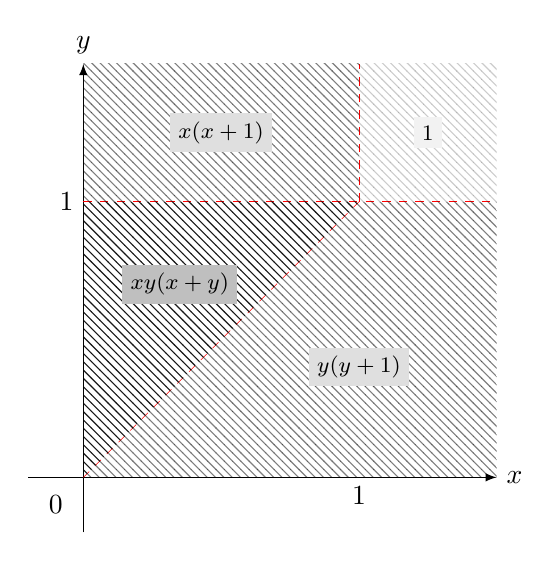
\begin{tikzpicture}[scale=3.5]
                \draw[-latex] (-0.2,0) -- (1.5,0) node[right] {$x$};
                \draw[-latex] (0,-0.2) -- (0,1.5) node[above] {$y$};
                \node[left] at (0,1) {$1$};
                \node[below] at (1,0) {$1$};

                \draw[very thin,red,dashed] (0,0) -- (1,1);
                \draw[very thin,red,dashed] (1,1) -- (1,1.5);
                \draw[very thin,red,dashed] (0,1) -- (1.5,1);

                \fill[gray,opacity=0.9,pattern=north west lines,line width=1pt] (0,0) -- (1,1) -- (0,1) -- cycle;
                \fill[gray,opacity=0.5,pattern=north west lines,line width=1pt] (0,1) -- (1,1) -- (1,1.5) -- (0,1.5) --cycle;
                \fill[gray,opacity=0.5,pattern=north west lines,line width=1pt] (0,0) -- (1,1) -- (1.5,1) -- (1.5,0) -- cycle;
                \fill[gray,opacity=0.2,pattern=north west lines,line width=1pt] (1,1) -- (1.5,1) -- (1.5,1.5) -- (1,1.5) -- cycle;

                \node at (0.35,0.7) {\footnotesize\colorbox{lightgray}{$xy(x+y)$}};
                \node at (0.5,1.25) {\footnotesize\colorbox{lightgray!50}{$x(x+1)$}};
                \node at (1.0,0.4) {\footnotesize\colorbox{lightgray!50}{$y(y+1)$}};
                \node at (1.25,1.25) {\footnotesize\colorbox{lightgray!20}{$1$}};
                \node at (-0.1,-0.1) {$0$};
            \end{tikzpicture} 
            \end{center}
            \[F(x,y)=\begin{cases}
                0 & \text{for } x<0\text{ or }y<0\\
                xy(x+y) & \text{for } 0\leq x\leq y\leq 1\\
                x(x+1) & \text{for } y>1,\quad 0\leq x\leq 1\\
                y(y+1) & \text{for } x\geq 0,\quad 0\leq y\leq x\leq 1\\
                1 & \text{for } x>1\text{ or }y>1
            \end{cases}\]
            \item Find the conditional pdf $f(y|x)$.\\
            \jawab
            \begin{flalign*}
                f(y|x)&=\frac{f(x,y)}{f_1(x)}&\\
                &=\frac{2x+2y}{1-3x^2},\quad 0\leq x\leq y\leq 1
            \end{flalign*}
            \item Find the conditional pdf $f(x|y)$.\\
            \jawab
            \begin{flalign*}
                f(x|y)&=\frac{f(x,y)}{f_2(y)}&\\
                &=\frac{2x+2y}{3y^2},\quad 0\leq x\leq y\leq 1
            \end{flalign*}
        \end{enumerate}
        \item[29.] Suppose $X$ and $Y$ are continuous random variables with joint pdf given by
        $f(x,y)=24xy$ if $0<x,\,0<y,\,x+y<1$ and zero otherwise.
        \begin{enumerate}
            \item Are $X$ and $Y$ independent? Why or why not?\\
            \jawab\\
            $X$ and $Y$ dependent because "support set" isn't cartesian product.
            \item Find $P[Y>2X]$.\\
            \jawab\\
            The probabilty and pdf region can be seen in the following figure.
            \begin{center}
                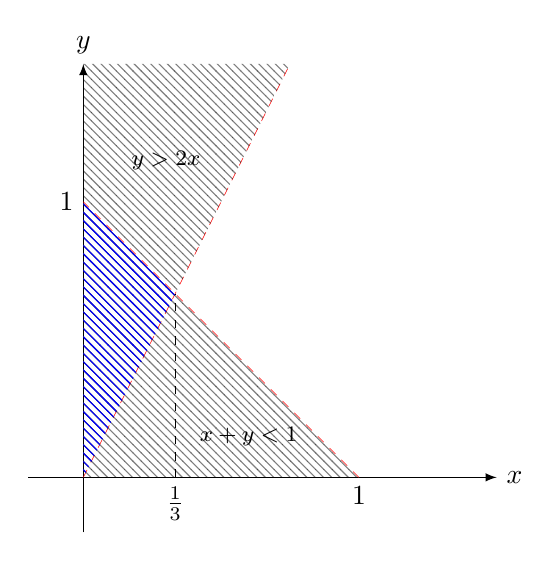
\begin{tikzpicture}[scale=3.5]
                    \draw[-latex] (-0.2,0) -- (1.5,0) node[right] {$x$};
                    \draw[-latex] (0,-0.2) -- (0,1.5) node[above] {$y$};
                    \node[left] at (0,1) {$1$};
                    \node[below] at (1,0) {$1$};
                    \node[below] at ({1/3},0) {$\frac{1}{3}$};

                    \node at (0.6,0.15) {\footnotesize$x+y<1$};
                    \node at (0.3,1.15) {\footnotesize$y>2x$};

                    \draw[very thin,red,dashed] (1,0) -- (0,1);
                    \draw[very thin,red,dashed] (0,0) -- (0.75,1.5);
                    \draw[very thin,dashed] ({1/3},0) -- ({1/3},{2/3});

                    \fill[gray,opacity=0.5,pattern=north west lines,line width=1pt] (0,0) -- (0,1) -- (1,0) --cycle;
                    \fill[gray,opacity=0.5,pattern=north west lines,line width=1pt] (0,0) -- (0.75,1.5) -- (0,1.5) -- cycle;
                    \fill[opacity=1,pattern=north west lines,pattern color=blue,line width=1pt] (0,0) -- ({1/3},{2/3}) -- (0,1) -- cycle;
                    \end{tikzpicture}
            \end{center}
            Hence, the probability can be calculated as following.
            \begin{flalign*}
                P[Y>2X]&=\int_0^{1/3}\int_{2x}^{1-x}24xy\,dy\,dx&\\
                &=\int_0^{1/3}\left[12xy^2\right]_{2x}^{1-x}\,dx&\\
                &=\int_0^{1/3}\left[12x(1-x)^2-12x(2x)^2\right]\,dx&\\
                &=\int_0^{1/3}\left[12x(1-2x+x^2)-48x^3\right]\,dx&\\
                &=\int_0^{1/3}\left[12x-24x^2+12x^3-48x^3\right]\,dx&\\
                &=\int_0^{1/3}\left[12x-24x^2-36x^3\right]\,dx&\\
                &=\left[6x^2-8x^3-9x^4\right]_0^{1/3}&\\
                &=6\left(\frac{1}{3}\right)^2-8\left(\frac{1}{3}\right)^3-9\left(\frac{1}{3}\right)^4&\\
                &=6\left(\frac{1}{9}\right)-8\left(\frac{1}{27}\right)-9\left(\frac{1}{81}\right)&\\
                &=\frac{6}{9}-\frac{8}{27}-\frac{9}{81}&\\
                &=\frac{2}{3}-\frac{8}{27}-\frac{1}{9}&\\
                &=\frac{18-8-3}{27}&\\
                &=\frac{7}{27}
            \end{flalign*}
            \item Find the marginal pdf of $X$.
            \begin{flalign*}
                f_1(x)&=\int_{-\infty}^\infty f(x,y)\,dy&\\
                &=\int_0^{1-x}24xy\,dy&\\
                &=\left[12xy^2\right]_0^{1-x}&\\
                &=12x(1-x)^2&\\
                &=12x(1-2x+x^2)&\\
                &=12x-24x^2+12x^3
            \end{flalign*}
        \end{enumerate}
    \end{enumerate}
\end{document}